$subject$=Физические основы компьютерных \\ и сетевых технологий
$teacher$=Лекции Зинчика А. А.
$date$=15.09.2025

Нормальной дисперсией считается дисперсия при $\frac{dn}{d\lambda_0} < 0$, то есть $v_{\text{гр}} < v_{\text{фаз}}$. В нормальной дисперсии с увеличением частоты света показатель преломления увеличивается

Аномальной дисперсией считается при $\frac{dn}{d\lambda_0} > 0$. Аномальная дисперсия была открыта позже и проявляется реже, поэтому при открытии казалась исключением из правила

\mediumvspace

Оценим воздействие электромагнитной волны на электроны. Сила Лоренца намного меньше силы Кулона из-за того, что скорость свободного электрона намного меньше скорость света:

$\frac{F_{\text{Лоренца}}}{F_{\text{Кулона}}} \sim \frac{v e B}{e E} \sim \frac{v \mu_0 H}{E} \sim v \sqrt{\varepsilon_0 \mu_0} = \frac{v}{c} \ll 1$

Поэтому рассмотрим электрон как совершающий вынужденные из-за силы Кулона колебания:

$\ddot x + 2 \beta \dot x + \omega_0^2 x = \frac{e E_0}{m_e} e^{i \omega t}$

Если дипольный момент электрона в веществе $p = -ex$, то поляризованность вещества $P = Np = -Nex$. Тогда $\ddot P + 2 \beta \dot P + \omega^2_0 P = \frac{e^2 N E_0}{m_e} e^{i \omega t}$

Пусть $P = P_0 e^{i \omega t}$, тогда $(-\omega^2 + 2 i \bta \omega + \omega_0^2) P_0 = \frac{e^2 N E_0}{m_e}$

Для линейной среды $P_0 = \varepsilon_0 (\varepsilon - 1) E_0$, получаем $\varepsilon = 1 + \frac{\omega_p^2}{\omega_0^2 - \omega^2 + 2i\beta \omega} = \varepsilon^{\prime} - i \varepsilon^{\prime\prime}$

$\omega_p^2 = \frac{e^2 N}{m_e \varepsilon_0}$ называют плазменной частотой. В электромагнитной волне с такой частотой электроны в веществе не успевают начать движение и остаются на месте

Если $\beta$ мало, то $\varepsilon^{\prime\prime} \ll \varepsilon^{\prime}$, значит корень можно представить в виде двух членов ряда Тейлора:

$n = \sqrt{\varepsilon} = \sqrt{\varepsilon^{\prime} \left(1 - \frac{i \varepsilon^{\prime\prime}}{\varepsilon^{\prime}}\right)} = n^{\prime} - i n^{\prime\prime}$

Если $\beta = 0$, то есть поглощения волн нет, то \fbox{$n = \sqrt{\varepsilon} = 1 + \frac{b}{\omega_0^2 - \omega^2}$}, где $b = \omega_p^2 = \frac{e^2 N}{m_e \varepsilon_0}$, $\omega_0$ -- собственная частота вещества, $\omega$ -- частота волны


\section{3. Тепловое излучение}

Тепловое излучение -- это испускание электромагнитных волн телами за счет их внутренней энергии

Тепловое излучения имеет место при любой температуре $T > 0$ К, но при невысоких температурах излучаются практически длинные (инфракрасные) электромагнитные волны

В начале развития металлургии кузнец на глаз могли определять температуру металла при ковке по его цвету. Лампа накаливания использует тепловое излучение. В ней раскаляется спираль из вольфрама, которая начинает излучать свет

Энергетическая светимость $R_{T}$ -- это энергия, испускаемая в единицу времени с единицы поверхности излучающего тела во всем интервале частот по всем направлениям

Спектральная плотность энергетической светимости (или испускательная способность) $r_{\omega T}$ -- это энергия, испускаемая в единицу времени с единицы поверхности излучающего тела в узком интервале частот от $\omega$ до $\omega + d \omega$. Очевидно, что $r_{\omega T} = \frac{d R_{\omega T}}{d \omega}$, тогда как $R_T = \int_0^\infty r_{\omega T} d\omega$

Поглощательная способность $\alpha_{\omega T}$ -- это отношение поглощенного телом потока лучистой энергии к падающему потоку этой энергии, заключенному в узком интервале частот от $\omega$ до $\omega + d\omega$. Поглощательная способность вычисляется как $\alpha_{\omega T} = \frac{d \Phi_{\text{погл}}}{d \Phi_{\text{пад}}}$

Если $\alpha_{\omega T} = 1$ для всех частот и температур, то тело называется абсолютно черным. Аналогично, абсолютно белое тело -- тело, для которого $\alpha_{\omega T} = 0$. Серое тело - тело, для которого $\alpha_{\omega T} = \const < 1$

\mediumvspace

% https://www.geogebra.org/calculator/bxcq8gdq

\begin{wrapfigure}{R}{0pt}
    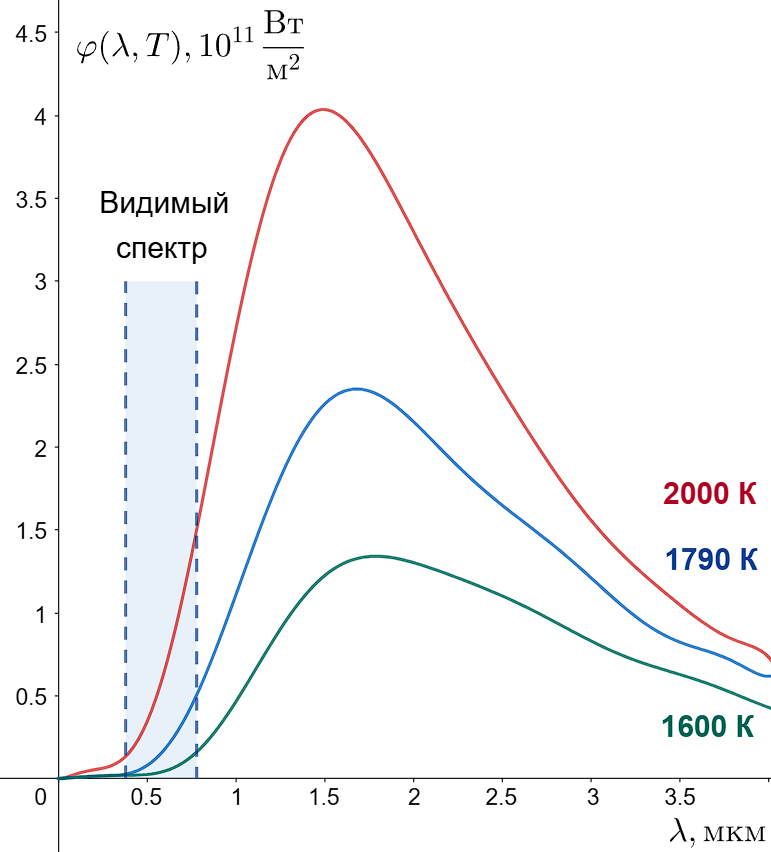
\includegraphics[width=7cm]{physics3/images/physics3_kirchhoff_law_functions}
\end{wrapfigure}

Физик Густав Кирхгофа на основе наблюдений выразил закон Кирхгофа: отношение испускательной и поглощательной способности не зависит от природы тела, оно является для всех тел одной и той же функцией частоты и температуры

\[\left(\frac{r_{\omega T}}{\alpha_{\omega T}}\right)_1 = \left(\frac{r_{\omega T}}{\alpha_{\omega T}}\right)_2 = \dots = \left(\frac{r_{\omega T}}{\alpha_{\omega T}}\right)_n = f(\omega, T)\]

Для абсолютно черного тела $f(\omega, T) = r_{\omega T}$

Далее экспериментально были получены кривые функций $\varphi(\lambda, T) = f\left(2\pi \frac{c}{\lambda}, T\right)$ для разных температур для абсолютно черного тела

На ней можно заметить, что при высоких температурах (2300 - 3100 К) лишь малая часть теплового излучения лежит в видимом для человека спектре, что объясняет малый КПД лампы накаливания


Позже был сформулирован закон Стефана-Больцмана: $R_T = \int_0^\infty r_{\omega T} d\omega = \int_0^\infty f(\omega, T) d\omega = \sigma T^4$, где $\sigma = 5.67 \cdot 10^{-8} \frac{\text{Вт}}{\text{м}^2 \cdot \text{К}^4}$ -- постоянная Стефана-Больцмана

Таким образом, можно вычислить мощность света от Солнца, попадающего на квадратный метр площадки на Земле и получить примерно $130 \frac{\text{Вт}}{\text{м}^2}$

Из этого появился закон Вина, который гласит, что максимум спектральной плотности энергетической светимости обратно пропорционален абсолютной температуре $\lambda_{\max} = \frac{b}{T}$, где $b = 2.9 \cdot 10^{-3} \text{м}\cdot\text{К}$ -- постоянная Вина

Функцию $f(\omega, T)$ пытались представить аналитически. Физики Рэлей и Джинс сформировали формулу Рэлея-Джинса: $f(\omega, T) = \frac{\omega^2}{4\pi^2 c^2} kT$. Эта формула хорошо сходится для больших длин волн, но плохо для маленьких в ультрафиолетовом спектре, так как $\int_0^\infty \frac{\omega^2}{4\pi^2 c^2} kT d\omega = \infty$ -- этот результат получил название ультрафиолетовой катастрофы

Позже Макс Планк высказал гипотезу Планка: электромагнитное излучение испускается телами не непрерывно, а в виде отдельных порций энергии (квантов), величина которых равна 

\[\varepsilon = h \nu = \frac{h c}{\lambda} = \hbar \omega,\]

где $h = 6.63 \cdot 10^{34} \text{Дж}\cdot\text{с}$ -- постоянная Планка, $\hbar = \frac{h}{2\pi} = 1.05 \cdot 10^{34} \text{Дж}\cdot\text{с}$ -- постоянная Планка с чертой

Энергия излучения получается, как сумма порций энергий $\varepsilon_n = n \hbar \omega$, где $n \in \Natural$

Далее Планк описал формулу спектральной плотности излучения абсолютно черного тела:

\[r_{\omega T} = \frac{\hbar \omega^3}{4 \pi^2 c^2} \frac{1}{e^{\frac{h\nu}{kT}} - 1}\]

Или для спектральной плотности от длины волны:

\[r_{\lambda T} = \frac{2 h c^2}{\lambda^5} \frac{1}{e^{\frac{hc}{\lambda kT}} - 1}\]

При $\frac{\hbar \omega}{kT} \gg 1$ (область высоких частот) получаем $f(\omega, T) = \frac{\omega^3}{4\pi^2 c^2} \frac{1}{1 + \frac{\hbar \omega}{kT} - 1} = \frac{\omega^3}{4\pi^2 c^2} kT$ -- формула Рэлея-Джинса

При $\frac{\hbar \omega}{kT} \ll 1$ (область низких частот) получаем $f(\omega, T) = \frac{\omega^3}{4\pi^2 c^2} e^{-\frac{\hbar \omega}{k T}} = \omega^2 \cdot F\left(\frac{\omega}{T}\right)$ -- формула Вина

Для абсолютно черного тела $R_T = \int_0^\infty \frac{\hbar}{4\pi^2 c^2} \frac{\omega^3 d\omega}{e^{-\frac{\hbar \omega}{k T}} - 1} = \frac{\pi^2 k^4}{60 c^2 \hbar^3} T^4 = \sigma T^4$ -- закон Стефана-Больцмана

\smallvspace 

Исследуем формулу Планка на экстремум, возьмем $\frac{d \varphi(\lambda, T)}{d\lambda} = 0$, получим трансцендентное уравнение $x e^x - 5(e^x - 1) = 0$, решением которого является $\frac{2\pi \hbar c}{k T \lambda_{\max}} = 4.965$, отсюда получаем закон смещения Вина: $T \lambda_m = \frac{2\pi \hbar c}{4.965 k} = b$

\bigvspace

Фотоэффект -- эффект, при котором электроны двигаются в веществе под действием светового излучения

Различают 3 типа фотоэффекта:

\begin{itemize}
    \item Внешний -- электрон покидает вещество. На основе внешнего фотоэффекта работают фотоэлементы
    
    Внешний фотоэффект создается так: помещаются фотокатод и анод в прозрачную колбу и откачивают воздух. При попадании света на фотокатод электроны переносятся с него на анод, создавая ток 

    \item Внутренний -- перераспределение электронов внутри чистого полупроводника под действием света. На внутреннем фотоэффекте основаны фоторезисторы

    \item Вентильный -- пропускание электроном через p-n переход при его обратном включении под действием света. На основе этого фотоэффекта работают фотодиоды
\end{itemize}


Наблюдения помогли понять, что при определенной длины волны фотоэффект резко прекращается. Чтобы выбить электрон из кристаллической решетки наружу, нужно сообщить ему энергию

Основные закономерности внешнего фотоэффекта отражены зависимостью величины фототока от напряжения между анодом и катодом. Такая зависимость называется вольт-амперной характеристикой: $I = I(U)$

% TODO картинка ВАХ

На вольт-амперной характеристике можно заметить две точки:

\begin{itemize}
    \item Напряжение, при котором тока нет. Его называют задерживающим (или запирающим) и оно обратного направления
    \item Ток насыщения, при котором выбивается максимально возможное число электронов из пластинки
\end{itemize}

\mediumvspace

Далее явление фотоэффекта изучал Столетов, который сформулировал первый закон фотоэффекта: сила фототока насыщения пропорциональная падающему световому потоку, то есть $I = \Phi$

Величина задерживающего напряжения позволяет определить максимальную скорость электронов

Второй закон фотоэффекта гласит, что задерживающее напряжение прямо пропорционально зависит от частоты: $U_\text{зап} = a\nu + b$, то есть $\tg \alpha = a = \const$

Третий закон фотоэффекта утверждает, что для каждого металла существует минимальная частота $\nu_{\text{кр}}$, при которой начинается фотоэффект

Часто длина волны такой частоты является красной, поэтому ее называют красной границей фотоэффекта

Разные металлы имеют различную частоту красной границы и одинаковую зависимость задерживающего напряжения от частоты

\mediumvspace

В 1905 году Альберт Эйнштейн объяснил второй закон тем, что металл поглощает свет порциями, то есть квантами. Тогда по формуле Планка $\varepsilon_{\text{фотона}} = h \nu$ получаем:

\fbox{$h \nu = A_{\text{выхода}} + E_{\text{кин. элект.}} = A_{\text{выхода}} + \frac{m v^2_{\max}}{2}$} -- уравнение Эйнштейна для фотоэффекта

\smallvspace

Здесь $A_{\text{выхода}}$ -- работа выхода, необходимая энергия для вытеснения электрона из вещества при температуре абсолютного нуля. Работа выхода для многих металлов находится в интервале от 1 до 10 эВ

При $v_{\max}$ получаем $\nu_\text{кр} = \frac{A_\text{вых}}{h}$

Также можем представить второй закон фотоэффекта так: $U_\text{зап} = \frac{h}{e} \nu - \frac{A_\text{вых}}{e}$
